\documentclass[tikz,border=2pt]{standalone}
\usepackage{amsmath,amssymb}
\usetikzlibrary{arrows.meta}
\begin{document}
% Bag with 6 red and 3 blue balls. With replacement the drawn ball goes back and the next draw
% is red with probability 6/9 again; without replacement the bag shrinks and, after a red draw,
% the next draw is red with probability 5/8.
\newcommand{\ball}[3]{\filldraw[fill=#3!30, draw=#3!70!black, thick] (#1,#2) circle (0.15);}
% \bag{x}{y}{number of red balls}: 3 x 3 layout, red first, then 3 blue; missing red balls dashed
\newcommand{\bag}[3]{%
  \draw[gray, rounded corners=6pt, thick] (#1-0.35,#2+0.35) rectangle (#1+1.25,#2-1.25);%
  \foreach \k in {0,...,5} {%
    \pgfmathtruncatemacro{\r}{int(\k/3)}\pgfmathtruncatemacro{\c}{mod(\k,3)}%
    \ifnum\k<#3 \ball{#1+0.45*\c}{#2-0.45*\r}{red}%
    \else \draw[gray, dashed] (#1+0.45*\c,#2-0.45*\r) circle (0.15);\fi}%
  \foreach \c in {0,1,2} {\ball{#1+0.45*\c}{#2-0.9}{blue}}}
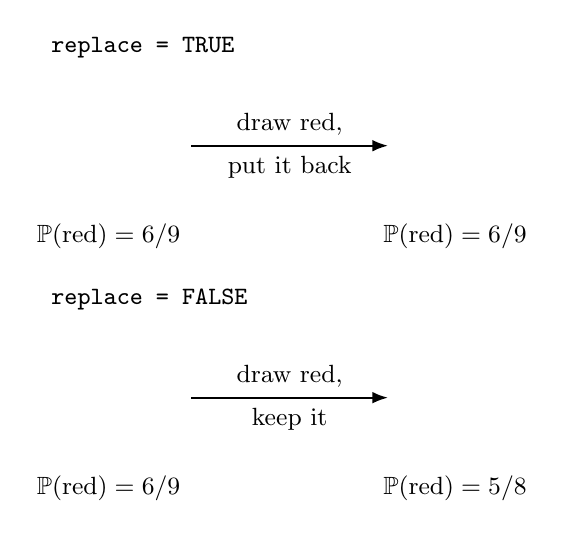
\begin{tikzpicture}[font=\small, >={Latex[length=2mm]}]
  % with replacement
  \node[anchor=west] at (-0.4,0.8) {\texttt{replace = TRUE}};
  \bag{0}{0}{6}
  \draw[->, thick] (1.5,-0.45) -- node[above] {draw red,} node[below] {put it back} (4.0,-0.45);
  \bag{4.4}{0}{6}
  \node at (0.45,-1.6) {$\mathbb{P}(\text{red})=6/9$};
  \node at (4.85,-1.6) {$\mathbb{P}(\text{red})=6/9$};
  % without replacement
  \begin{scope}[yshift=-3.2cm]
  \node[anchor=west] at (-0.4,0.8) {\texttt{replace = FALSE}};
  \bag{0}{0}{6}
  \draw[->, thick] (1.5,-0.45) -- node[above] {draw red,} node[below] {keep it} (4.0,-0.45);
  \ball{2.75}{0.3}{red}
  \bag{4.4}{0}{5}
  \node at (0.45,-1.6) {$\mathbb{P}(\text{red})=6/9$};
  \node at (4.85,-1.6) {$\mathbb{P}(\text{red})=5/8$};
  \end{scope}
\end{tikzpicture}
\end{document}
